%   % !TEX root = ../../VIII,3_Rahmen-TeX_9-0.tex
%  
%   Signatur/Tex-Datei:	LH_37_05_162r
%   RK-Nr. 	57266_2		(_1 und _3 auf demselben Träger)
%   Titel: 			Propositio fundamentalis totius scientiae Mechanicae
%   Datierung:		März-Mai 1677 										??
%   WZ: 			keins
%   Diagramme: 		1
%   Dateien (PDF):
%   		LH_37_05_162r_d1
%
%
%
%
\selectlanguage{ngerman}
\frenchspacing
%
\begin{ledgroupsized}[r]{120mm}
\footnotesize
\pstart
\noindent\textbf{Überlieferung:}
\pend
\end{ledgroupsized}
%
\begin{ledgroupsized}[r]{114mm}
\footnotesize
\pstart \parindent -6mm
\makebox[6mm][l]{\textit{L}}%
Konzept: LH~XXXVII~5, Bl.~162.
Ein~Blatt~2\textsuperscript{o};
Papierschaden an den Rändern;
Papiererhaltungsmaßnahmen.
Eine Viertelseite auf Bl.~162~r\textsuperscript{o};
der obere Bereich von Bl.~162~r\textsuperscript{o} überliefert den Schlussteil von N.~\ref{57266_1}, Bl.~162~v\textsuperscript{o} überliefert N.~\ref{57266_3}.
Vermutlich bildete der Träger ursprünglich einen Bogen mit LH~XXXVII~5, Bl.~161.
\pend
\end{ledgroupsized}
%
\begin{ledgroupsized}[r]{114mm}
\footnotesize
\pstart
\parindent -6mm
\makebox[6mm][l]{\textit{E}}%
(tlw.) \cite{01056}\textsc{Fichant} 1994, S.~352.
\pend%
\end{ledgroupsized}
%
%
\vspace{5mm}
\begin{ledgroup}
\footnotesize
\pstart
\noindent%
\textbf{Datierungsgründe:}
Das vorliegende Stück wird unmittelbar im Anschluss an N.~\ref{57266_1} überliefert, das Leibniz eigenhändig auf März 1677 (a.\ St.)\ datiert hat, weist aber Unterschiede im Schreibduktus und in der Feder auf.
%
Die Rückseite desselben Blattes überliefert wiederum N.~\ref{57266_3}, das sich auf den Zeitraum März bis Mai 1677 (a.\ St.)\ datieren lässt. 
%
Unter der Annahme einer durchgehenden Beschreibung des Bogens, die durch die thematischen Überschneidungen der Stücke bekräftigt wird,
%
kann N.~\ref{57266_2} ebenfalls auf den Zeitraum März bis Mai 1677 (a.\ St.) datiert werden, jedoch vor N.~\ref{57266_3}.
\pend
%
\end{ledgroup}
%
%
\selectlanguage{latin}
\frenchspacing
% \newpage%
\vspace{8mm}
\pstart%
\normalsize%
\noindent%
\edtext{\lbrack162~r\textsuperscript{o}\rbrack\ Propositio}{
\lemma{\lbrack162~r\textsuperscript{o}\rbrack}%
\Bfootnote{%
\textit{(1)}~Duae propositiones fundamentales totius scientiae %
\textit{(a)}~de Motu: E 
\textit{(b)}~Mechanicae: 
(1)~ eadem semper manet potentia \textbar\ seu vis \textit{gestr.}\ \textbar\ (2) eadem semper manet %
\textit{(aa)}~directio %
\textit{(bb)}~determin  %
\textit{(cc)}~directio. %
\textit{(2)}~Propositio~\textit{L}}}
%
fundamentalis totius scientiae
%
\edtext{Mechanicae:%
\protect\index{Sachverzeichnis}{scientia Mechanicae}%
\protect\index{Sachverzeichnis}{propositio fundamentalis totius scientiae Mechanicae} Datis corporibus}
{\lemma{Mechanicae}\Bfootnote{%
\textit{(1)}~Sumto quodam corporum aggregato nihil ab extrinseco 
\textbar\ in \textit{streicht Hrsg.}~\textbar\ 
\textit{(2)}~Datis \textit{(a)}~aliquot \textit{(b)}~corporibus~\textit{L}}}
%
\edtext{quotcunque nihil ab aliis}
{\lemma{quotcunque}\Bfootnote{%
\textit{(1)}~nihi  \textit{(2)}~quae nihil ab aliis pati intelli
\textit{(3)}~ab \textit{(4)}~nihil \textit{(a)}~aliunde \textit{(b)}~aliunde \textit{(c)}~ab
\textit{(aa)}~extrinseci \textit{(bb)}~aliis~\textit{L}}}
%
extra
%
\edtext{ipsa sumtis}{\lemma{ipsa}\Bfootnote{%
\textit{(1)}~patientibus \textit{(2)}~sumtis~\textit{L}}}
%
patientibus, eadem semper manet %
potentia\protect\index{Sachverzeichnis}{potentia} et %
directio\protect\index{Sachverzeichnis}{directio} totius aggregati.%
\protect\index{Sachverzeichnis}{potentia totius aggregati}%
\protect\index{Sachverzeichnis}{directio totius aggregati}
%
\textso{Potentia}%
\protect\index{Sachverzeichnis}{potentia} est quantitas
effectus,%
\protect\index{Sachverzeichnis}{quantitas effectus} quem res aliqua producere potest. Directio%
\protect\index{Sachverzeichnis}{directio} est linea motus,%
\protect\index{Sachverzeichnis}{linea motus} vel si curva sit ejus tangens;
directio totius 
% [?]
aggregati%
\protect\index{Sachverzeichnis}{directio totius aggregati} eadem est quae directio centri gravitatis.%
\protect\index{Sachverzeichnis}{directio centri gravitatis}%
\protect\index{Sachverzeichnis}{centrum gravitatis} Nulla enim alia totius %
directio\protect\index{Sachverzeichnis}{directio} intelligi potest.
In aggregato corporum quotcunque sibi relicto%
\protect\index{Sachverzeichnis}{aggregatum corporum sibi relictum} eadem semper %
potentia et 
\edtext{directio totius}{\lemma{directio}\Bfootnote{\textit{(1)}~conservatur \textit{(2)}~totius~\textit{L}}}
aggregati%
\protect\index{Sachverzeichnis}{potentia totius aggregati}%
\protect\index{Sachverzeichnis}{directio totius aggregati} servatur. Cum enim sibi relictum esse intelligamus, nihil est quod mutet.  Servatur ergo %
potentia\protect\index{Sachverzeichnis}{potentia} et
%
directio\protect\index{Sachverzeichnis}{directio} non quidem partium,%
\protect\index{Sachverzeichnis}{directio partium}%
\protect\index{Sachverzeichnis}{potentia partium} eae enim invicem patiuntur, augentque et minuunt potentiam, et mutant 
directionem; sed totius. Est autem %
directio totius\protect\index{Sachverzeichnis}{directio totius} eadem quae directio certi alicujus puncti. Quod semper
progredi necesse est.
\pend
%
\vspace{2.0em} %%%%%%%%% Diagramm 1
\centerline{%
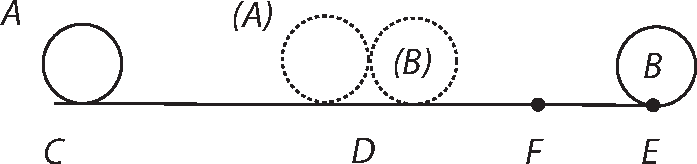
\includegraphics[width=0.55\textwidth]{%
gesamttex/edit_VIII,3/images/LH_37_05_162r_d1.pdf%
}} 
\vspace{0.5em}
\centerline{%
\lbrack\textit{Fig.~1}\rbrack%
}
% \newpage%
\vspace{1.5em}
%
\pstart
Sit corpus \textit{A}, ejus celeritas $a\,\sqcap\,CD$\lbrack,\rbrack\ corpus \textit{B}, ejus celeritas $b\,\sqcap\,DE$\lbrack,\rbrack\
distantia corporum $a+b \, \sqcap\ CE$, %
punctum concursus\protect\index{Sachverzeichnis}{punctum concursus} \textit{D}. Sit %
centrum gravitatis\protect\index{Sachverzeichnis}{centrum gravitatis} 
\edtext{\lbrack\textit{F}\rbrack}{\lemma{}\Bfootnote{\textit{E} \textit{\ L ändert Hrsg.}}}. 
Erit 
$CF\,\sqcap\,B$. et $FE\,\sqcap\,A$. %
\pend